\chapter{Models Evaluated}

\section{Wilson}
The basis for the model is the Ph.D. dissertation of Joshua Wilson (\referencename~\cite{ref:wilson2017a}).  The model was further developed at Scientific Drilling.  It is a full featured stiff-string model based on the finite element method.  It includes coupled flexibility of the drill string, geometric nonlinearity, wellbore contact, fluid mass, and damping from fluid, amongst other features.

The full featured model is not open-source.  Instead, a limited version has been released to the \osdc{}.  Specifically, it has the following limitations.
\begin{bulletedlist}
	\item Straight wellbores only
	\item Constant wellbore OD
	\item No buckling
	\item No dynamic calculations
	\item Graphic user interfaces have been removed
	\item Advanced plotting features have been removed
\end{bulletedlist}
Specifically, since the dynamics have been removed, this model was not considered fit for purpose.

\section{Tulsa University Models}
Two models from Tulsa University were evaluated.  The source code for these models is available to CNPC USA through the TUDRP program. Ultimately, neither were selected for further evaluation.  The reviews of each and reasoning for not selecting them are presented below.

\subsection{Lateral Whirl Model}
The Ph.D. dissertation of Kriti Singh (\referencename~\cite{ref:singh2019a}) presents a model for lateral dynamics (whirl) of drill strings.

Dynamics are calculated in terms of Euler-Bernoulli beam elements and the solution is the general solution to the differential equation.

The Dynamic Transfer Matrix Simulator can be used to calculate the response of the BHA assembly to the specified excitation, for the specified RPM, WOB, and other operating parameters.

For the Dynamics Transfer Matrix Simulator it is assumed that if the deflection is larger than the borehole clearance, backward whirl will occur.

Primarily used to predict whirl in the drill string.

The numerical calculation is based on a single mass rotation disk.  This would only allow capturing the first natural frequency.

\notfinished{}


\subsection{Soft String Model}
The soft string model from Tulsa University is originally based on \referencename~\cite{ref:miska2015a} where the model was originally developed.  This model is ``dynamic'' in the sense that it incorporates inertia effects.  This is an improvement on other models which are purely static.

\notfinished{}

\cite{ref:zamanipour2018a}

In this paper, a dynamic, axially-stiff string model is presented for force calculations of drillstring in tripping operations.

Uses lumped mass and spring system.

Claims to be an axial stiff string model.  Allows for the string to be at the top or bottom of the hole automatically.  It does not seem to account for the no contact case.
Uses a 2D wellbore.

Static friction and drilling fluid drag are accounted for.

Input a top drive axial velocity and predict surface displacement, bottom velocity, bottom displacement, and hook load.

Compares axial ``stiff string'' model to a ``soft string'' model.  It seems that ``dynamic'' and ``static'' would be better nomenclature for these models.

\section{ExxonMobil Dixit Model}

\notfinished{}
\section{RGD model}

This section briefly summarizes the workflow of RGB model written in MATLAB. More detail description can be seen in Zhang and Detournay, 2020.\\ This code is for symmetric full blade which is defined as D1 bit in the paper.
The code calculates coupled PDE and ODE by solving the matrix
\begin{equation}\label{matrix}
  \bm{Adx} + \bm{BX} = \bm{Q}
\end{equation}

where $\bm{dx}$ and $\bm{X}$ are defined as follow:

\noindent\begin{minipage}{.5\linewidth}
\begin{equation}
\bm{x}=
\begin{bmatrix}
\dot{u} \\
u \\
\psi \\
\dot{\psi} \\
a_1\ \\
\vdots \\
a_N \\
\end{bmatrix}
\end{equation}
\end{minipage}%
\begin{minipage}{.5\linewidth}
\begin{equation}
\bm{dx}=
\begin{bmatrix}
\ddot{u} \\
\dot{u} \\
\dot{\psi} \\
\ddot{\psi} \\
\dot{a_1}\ \\
\vdots \\
\dot{a_N} \\
\end{bmatrix}
\end{equation}
\end{minipage} \\

 The bit trajectory function which is $\overline{h}(\tau, \theta$) is introduced and PDE can be derived from equation:
\begin{equation}\label{PDE}
\frac{\partial \overline{h}}{\partial \tau} + (w_0 + \dot{\psi})\frac{\partial \overline{h}}{\partial \theta}-v_0 = 0
\end{equation}

Equation (\ref{PDE}) is solved by Galerkin-method which approximates $\overline{h}(\tau, \theta$) by using base functions $a_1, a_2, ..., a_N$ (N=25 as default), where $\tau$ is scaled time and $\theta$ is rotation angle of the bit blade. The base functions can be obtained by minimizing the residual which are shown below (please note that all the derivations are for D1-bit):

\begin{equation}\label{GM}
\begin{split}
R &= \left(\frac{n \theta}{2 \pi}-1\right)\dot{u}_b + \frac{n \theta}{2 \pi}\dot{a}_1 + \sum_{k=1}^{N-1}\dot{a}_{k+1}sin\left(\frac{nk\theta}{2}\right) \\ + &(w_0 + \dot{\psi}_0)\left[u_b\frac{n}{2\pi}+a_1\frac{n}{2\pi} + \sum_{k=1}^{N-1}\frac{a_{k+1}nk}{2}cos\left(\frac{nk\theta}{2}\right)\right]
\end{split}
\end{equation}

where n is the number of bit blade. In the paper the blade number is divided to $n_i$, and $n_o$ that are number of inner blades and outer blades, respectively. However, the codes runs for D1 bit and it contains n instead of $n_i and n_o$.

Minimizing $R(\theta, \tau)$ can be acheived by making it orthogonal to the base functions over the domain $\theta \in \left[0, \frac{2\pi}{n_i}\right]$, which results in:

\begin{equation}\label{GM1}
 \int_{0}^{\frac{2\pi}{n}}R(\theta,\tau)\frac{n\theta}{2\pi}d\theta = 0
\end{equation}

and

\begin{equation}\label{GM2}
 \int_{0}^{\frac{2\pi}{n}}R(\theta, \tau)sin\left(\frac{n_im\theta}{2}\right)d\theta=0, m= 1,....,N-1
\end{equation}
where N is the number of Galerkin base functions.

Equation (\ref{GM1})-(\ref{GM2}) represent a system of N first order equations for $a_i, i=1,2,...,N$ that is

\begin{equation}\label{Norder}
  \dot{a}_i = \Phi_i(\dot{u}, u, a_1, ..., a_N), i=1,...,N.
\end{equation}

Which is coupled with the equation of motion (governing equation) which are:

\begin{equation}\label{GE1}
  \varpi-\varpi_0 = n(\delta_n - \lambda(g(\nu)) - \frac{2\pi v}{w_0}
\end{equation}

\begin{equation}\label{GE2}
  \Gamma-\Gamma_0 = n(\delta_n -\beta \lambda(g(\nu)) - \frac{2\pi v}{w_0}
\end{equation}

where $\delta_n$ is given as:

\begin{equation}\label{deltan1}
  \delta_n = \overline{h}\left(\frac{2\pi}{n}, n\right) + u(\tau)
\end{equation}

$\varpi$, $\Gamma$ represent scaled WOB, TOB, respectively,  $\beta$ is number characterizing bit/rock interaction (generally less than 1). v and w are the scaled axial and angular velocity, respectively that are

\begin{equation}\label{scaled_axial_ve}
  v = v_0 + \dot{u}
\end{equation}
\begin{equation}\label{scaled_angular_vel}
  w = w_0 + \dot{\psi}
\end{equation}

So far we have N+2 equations with N+4 unknowns ($u, \dot(u), \psi, \dot(\psi), a_1, ..., a_N$). and two additional equations are obtained from relationship below:

\begin{equation}\label{axial_dis_vel}
  \dot{u} = \frac{\partial u}{\partial \tau}
\end{equation}
\begin{equation}\label{angular_dis_vel}
  \dot{\psi} = \frac{\partial \psi}{\partial \tau}
\end{equation}

Finally we obtained N+4 equations for the same number of unknowns and represent as linear from of $\bm{Adx} + \bm{BX} = Q$. and solve the equation for given time interval. However, the discontinuity should be investigated every time step which affects the boundary condition from rock-bit interaction. The model classifies the discontinuity to three which are 1) normal drilling, 2) axial stick, and 3) bit bonce. Below summarizes the conditions for each mode:

\begin{equation}\label{drillingmodes}
  \begin{cases}
    Normal\,drilling, & \mbox{if $\delta_n > 0, w > 0$, and $v > 0$ }  \\
    Axial\, stick, & \mbox{if $\delta_n >0, w > 0$, and $v = 0$ } \\
    Bit\,bounce, & \mbox{if $\delta_n = 0$, and $w > 0$}
  \end{cases}
\end{equation}

\section{Normal drilling}
Normal drilling mode simplifies the equations (\ref{GE1}), and (\ref{GE2}) since g($\nu$) = 0 which can be represented as:

\begin{equation}\label{GE1_normaldrilling}
  \varpi-\varpi_0 = n\left(\delta_n - \frac{2\pi v}{w_0}\right)
\end{equation}

\begin{equation}\label{GE2_normaldrilling}
  \Gamma-\Gamma_0 = n\left(\delta_n - \frac{2\pi v}{w_0}\right)
\end{equation}

Also, the depth of cut (\ref{deltan1}) is reduced to:

\begin{equation}\label{deltan_normaldrilling}
  \delta_n = a_1 + u(\tau)
\end{equation}

Afterwards, equation (\ref{matrix}) can be solved with reduced equations from equations (\ref{GE1_normaldrilling}) - (\ref{deltan_normaldrilling})

\newpage
\section{Extended RGD model (Zhang and Detournay, 2022)}


This section summarizes the paper from Zhang and Detournay 2022, which is an extension of RGD model. The proposed model is a multi-degrees of freedom (MDOF) model of a rotary drilling system simulating axial-torsional self-excited vibrations induced by the bit/rock interactions. Figure \ref{model_develop_figure} illustrates the development of the RGD model.

\begin{figure}[ht]
  \centering
  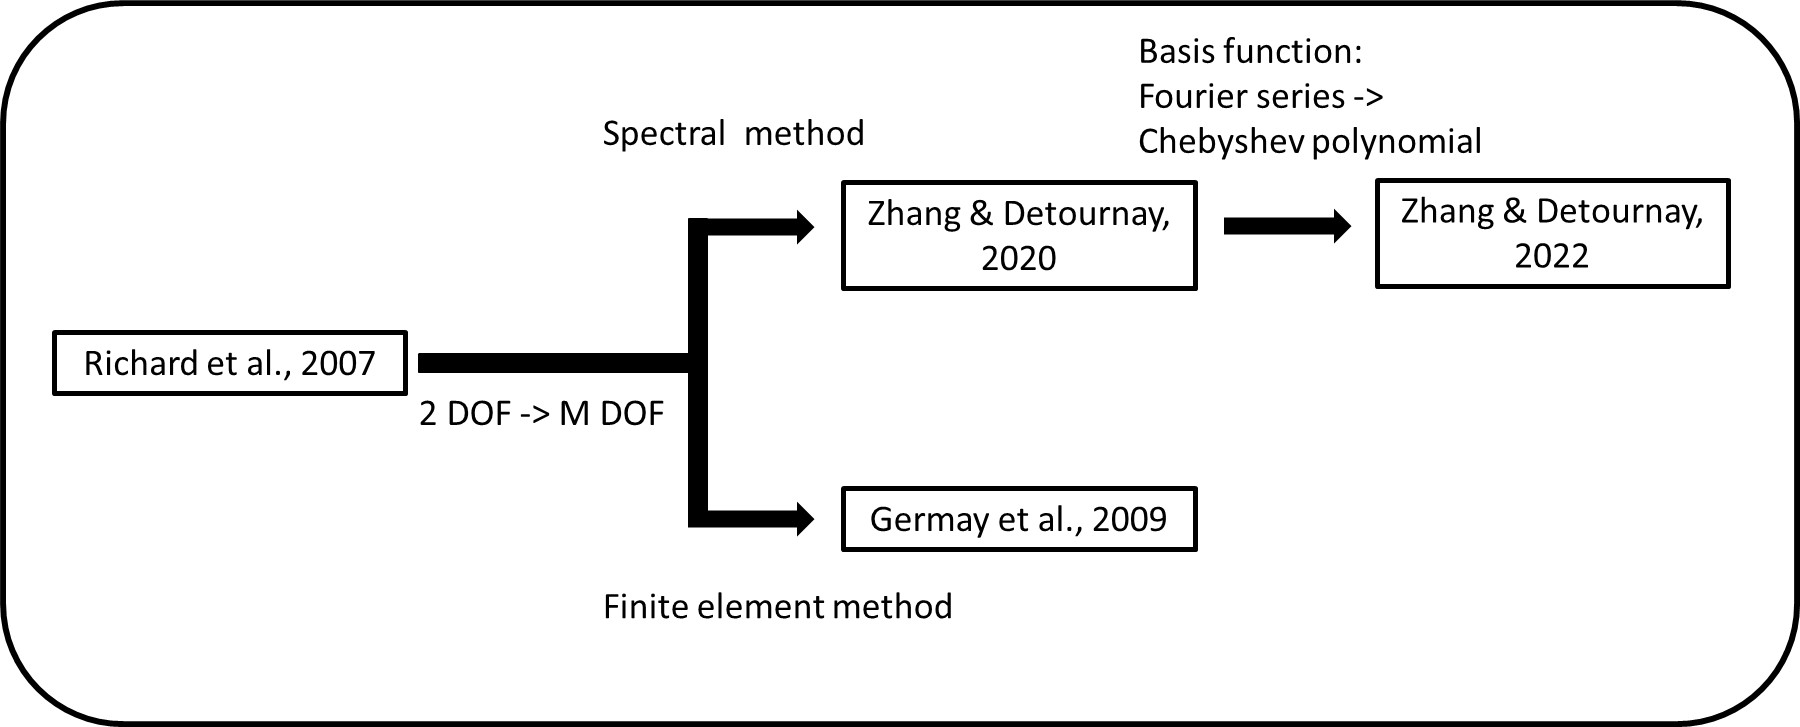
\includegraphics[width=5in]{ModelDevelop.jpg}
  \caption{RGD model development.}\label{model_develop_figure}
\end{figure}

The model represents the drillstring with multiple damped axial and torsional oscillators and the bit with symmetrically arranged blades. The schematic of MDOF model of the drillstring is shown in Figure \ref{MDOF_illustration}. The model takes into account damping and
different properties of drill pipe and BHA

\begin{figure}[ht]
  \centering
  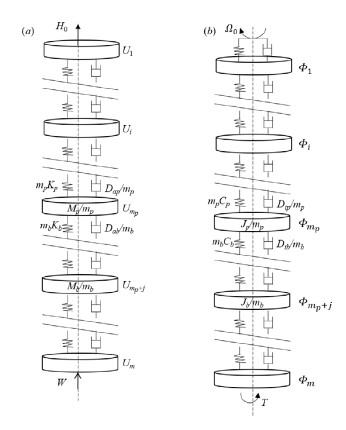
\includegraphics[height=3in]{MDOF_illustration.jpg}
  \caption{RGD model development.}\label{MDOF_illustration}
\end{figure}

The following assumptions are made: 1) The borehole is vertical, 2) Lateral vibration of the drillstring are neglected, 3) axial and torsional damping are proportional to the length of drill pipes and BHA, 4) constant hook load and rotary speed from surface (surface boundary conditions). Additionally, the discontinuity of the boundary condition at the bit-rock interface is modeled by
five different regimes classified based on axial, angular velocities, and depth-of-cut, namely, 1) normal drilling, 2) axial stick, 3) loss of contact, 4) torsional stick, 5) backward rotation

The system equations (PDE-ODE coupled) are established from equation of motions (axial and torsional), and bit trajectory function, which is defined to project depth of cut from the angular displacement of the bit. Then,
The PDE-ODE coupled system is numerically solved by discretizing the PDE-ODEs into ODEs. In this study, spectral method with Chebyshev polynomial is applied rather than finite element (FEM) or finite different method (FDM). Spectral method achieved high accuracy for a given number of basis functions and also converged faster compared to other numerical methods. (this is valid with simple geometry). \\

\noindent Some of the results and potential of the model are summarized below.
\begin{itemize}
  \item Modeling the vibrations of entire drillstring (not only the bit).
  \item Possible to conduct frequency analysis since it is multi-degrees of freedom model (Figure \ref{StickslipExample}).
  \item It can simulate axial and torsional vibrations including stick-slip event (Figure \ref{Axial_torsional_vibration_example}).
  \item Mode analysis can be done by computing the eigenvalues of the linearized system of equation.
  \item Computationally efficient compared to FEM assuming geometrically simple structure.
\end{itemize}

\begin{figure}[ht]
  \centering
  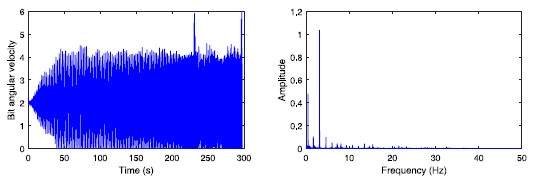
\includegraphics[width=6in]{StickslipExample.jpg}
  \caption{Simulation results of bit angular velocity and its frequency spectrum. The result shows the stick-slip occupance due to self-excited torsional vibration}\label{StickslipExample}
\end{figure}

\newpage

\begin{figure}[ht]
  \centering
  \includegraphics[height=5in]{Axial_torsional_vibration_example.jpg}
  \caption{Simulation results showing axial and angular velocity with scaled time. a) stable regime, b) slow regime of instability, c) fast regime of instability.}\label{Axial_torsional_vibration_example}
\end{figure}

\noindent The following are key questions or points that should be addressed for the model selection.
\begin{itemize}
  \item Can we model deviated or horizontal well?
  \item Geometrical nonlinearity in drillstring (for deviated well).
  \item Can we take int to account the effect of contact point?
  \item No lateral vibration - only modeling axial, torsional motion.
  \item Decoupling of axial and torsional vibration. this can be important when it comes to 3D model (i.e., whirling effect).
  \item Current code provided is 2 DOF model.
\end{itemize}







